\newpage
\section{Simulation Analysis}
\label{sec:simulation}
Since the input voltage source in this circuit is sinusoidal, the voltage and current values of the various components vary in time, and we are interested therefore in analysing how they evolve in time and obviously we want to picture the transformation of our AC input voltage source throughout the multiple stages of the circuit. Therefore, we will run a single transient analysis for this circuit, lasting 10 periods of the voltage source. For this simulation we are not taking the natural solution into account, only the forced one. In our simulation we came across a large transitional period of roughly 4 seconds, until the output voltage source stabilized enough in the envelope detector, so we only account for data after this period. This is due to the natural solution of the voltage and its downfall effects will be aproached in our conclusions. We used the default diode model of NGSpice in this simulation and we saw no need of introducing a transformer since it only reduces the amplitude of the voltage source, so we applied the AC voltage output of the transformer as our input voltage source of the circuit.
\subsection{Envelope Detector Output Voltage}
In figure~\ref{fig:envelope} we present the plot of the envelope detector output voltage throughout 10 periods, and in table~\ref{tab:envelope} we introduce the average voltage (approximate DC component) and the voltage ripple of such voltage. Since the objective lies in the output of the regulator, this set of data isn't of much relevance.

\begin{figure}[!h] \centering
\includegraphics[width=0.6\linewidth]{envelope.pdf}
\caption{Simulated output voltage in the envelope detector.}
\label{fig:envelope}
\end{figure}

\begin{table}[h]
  \centering
  \begin{tabular}{|l|r|}
    \hline    
    {\bf Name} & {\bf Values [V]} \\ \hline
    \input{env_tab} 
  \end{tabular}
  \caption{}
  \label{tab:envelope}
\end{table}

\subsection{Voltage Regulator Output Voltage - The output of the circuit}
In this section we simulate the natural response of the circuit in the [0,20] ms time interval using the transient analysis simulation in NGSpice and the computations from the previous section.
\begin{figure}[!h] \centering
\includegraphics[width=0.6\linewidth]{natura.pdf}
\caption{Simulated natural response for $V_{6}$ node voltage.}
\label{fig:natura}
\end{figure}
\newpage
\subsection{Natural and forced response}
We repeat the previous step now with the sinusoidal voltage source $V_{s}(t)$ considering a frequency of 1kHz. Below is the plot for both the stimulus and the response:
\begin{figure}[!h] \centering
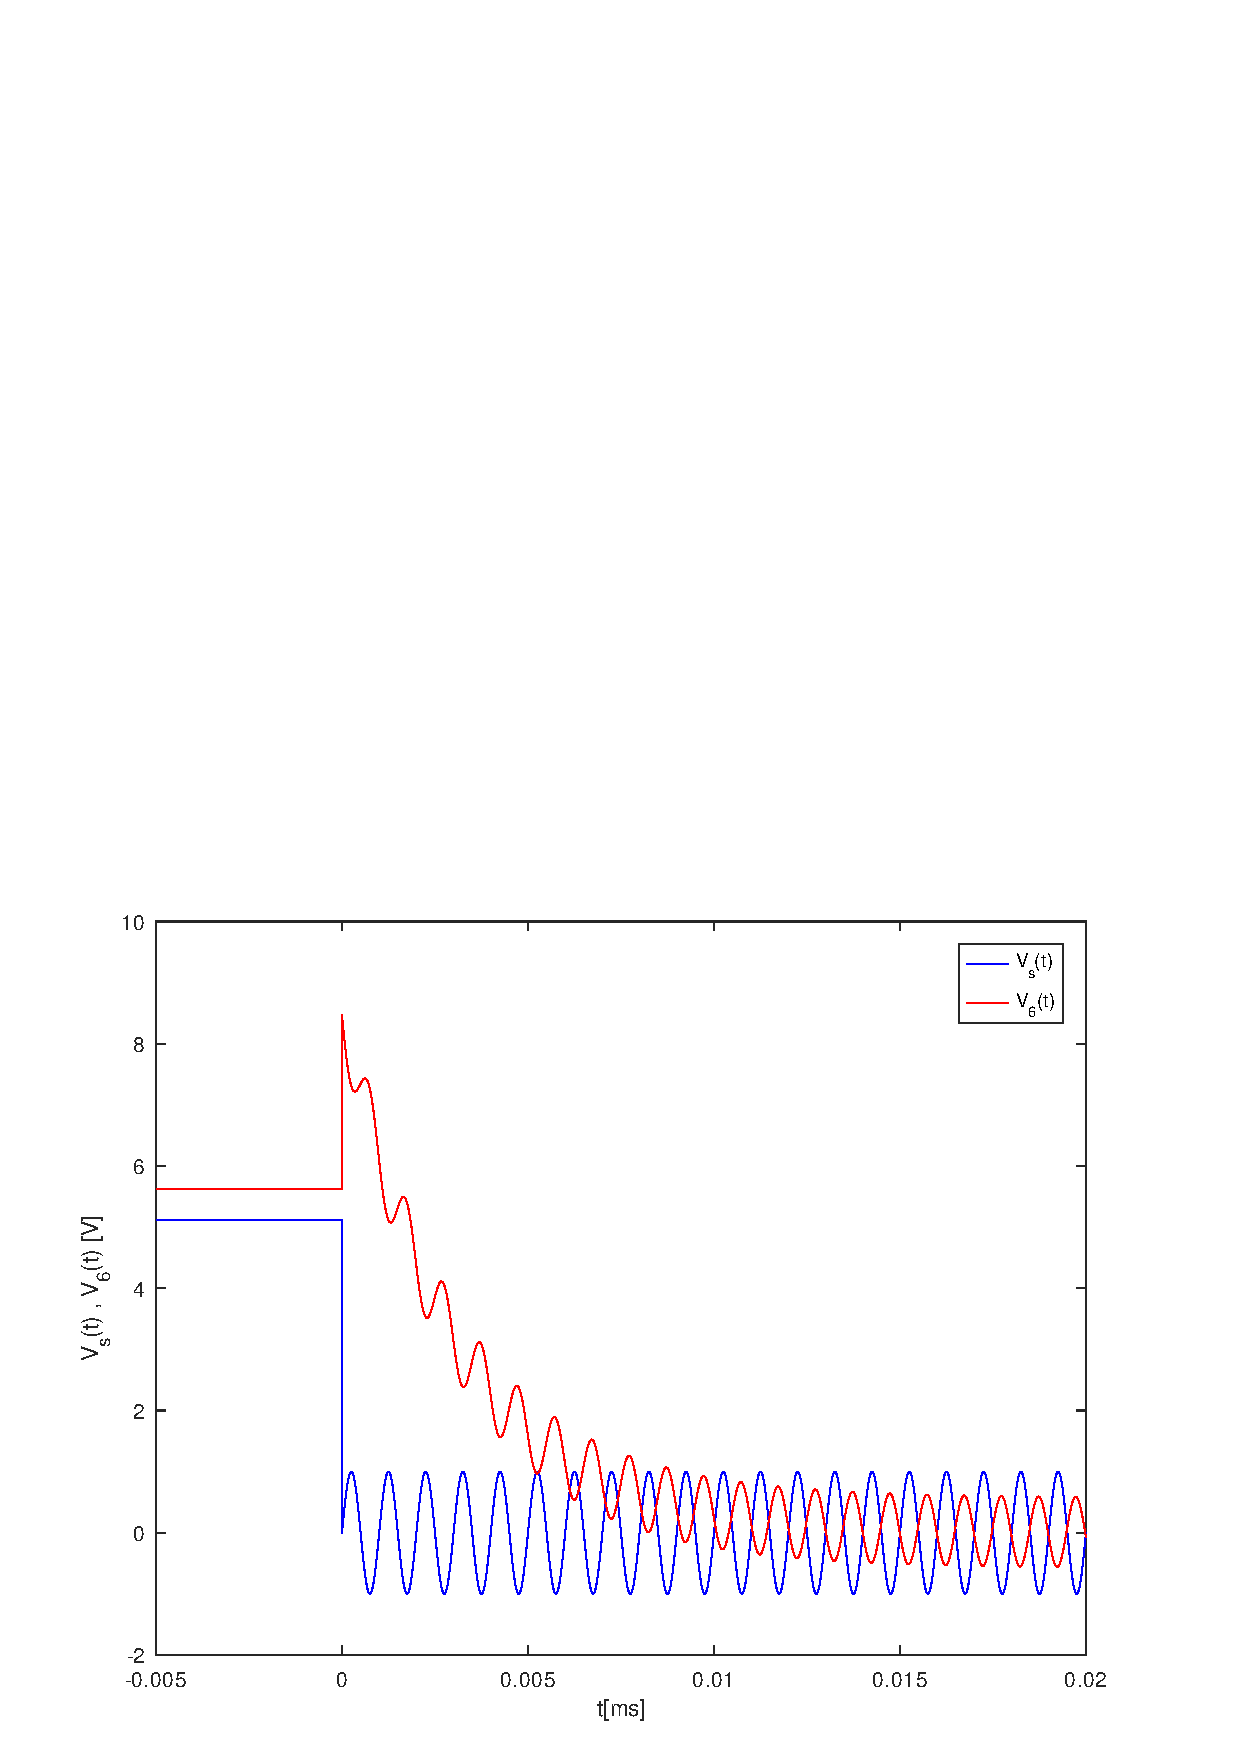
\includegraphics[width=0.6\linewidth]{total.pdf}
\caption{Simulated response for $V_{6}$ node voltage and stimulated voltage $V_{S}$.}
\label{fig:total}
\end{figure}
\newpage
\subsection{Frequency response}
We simulated the frequency response to the voltage source $V_{s}$, both in node 6 and in the capacitor itself, in NGSpice, and we plotted the magnitude, in dB, and phase, in degrees, of the three voltages in relation of course to a variation of frequency. The frequency varies from 0.1 Hz to 1MHz. Analysing figures ~\ref{fig:magnitude} and ~\ref{fig:phase}, they confirm what we foresaw in the theoretical analysis. The various reasons on why certain voltage parameters vary or are equivalent are laid out and explained in the $Frequency$ $Response$ subsection of the theoretical analysis.
\begin{figure}[!h] \centering
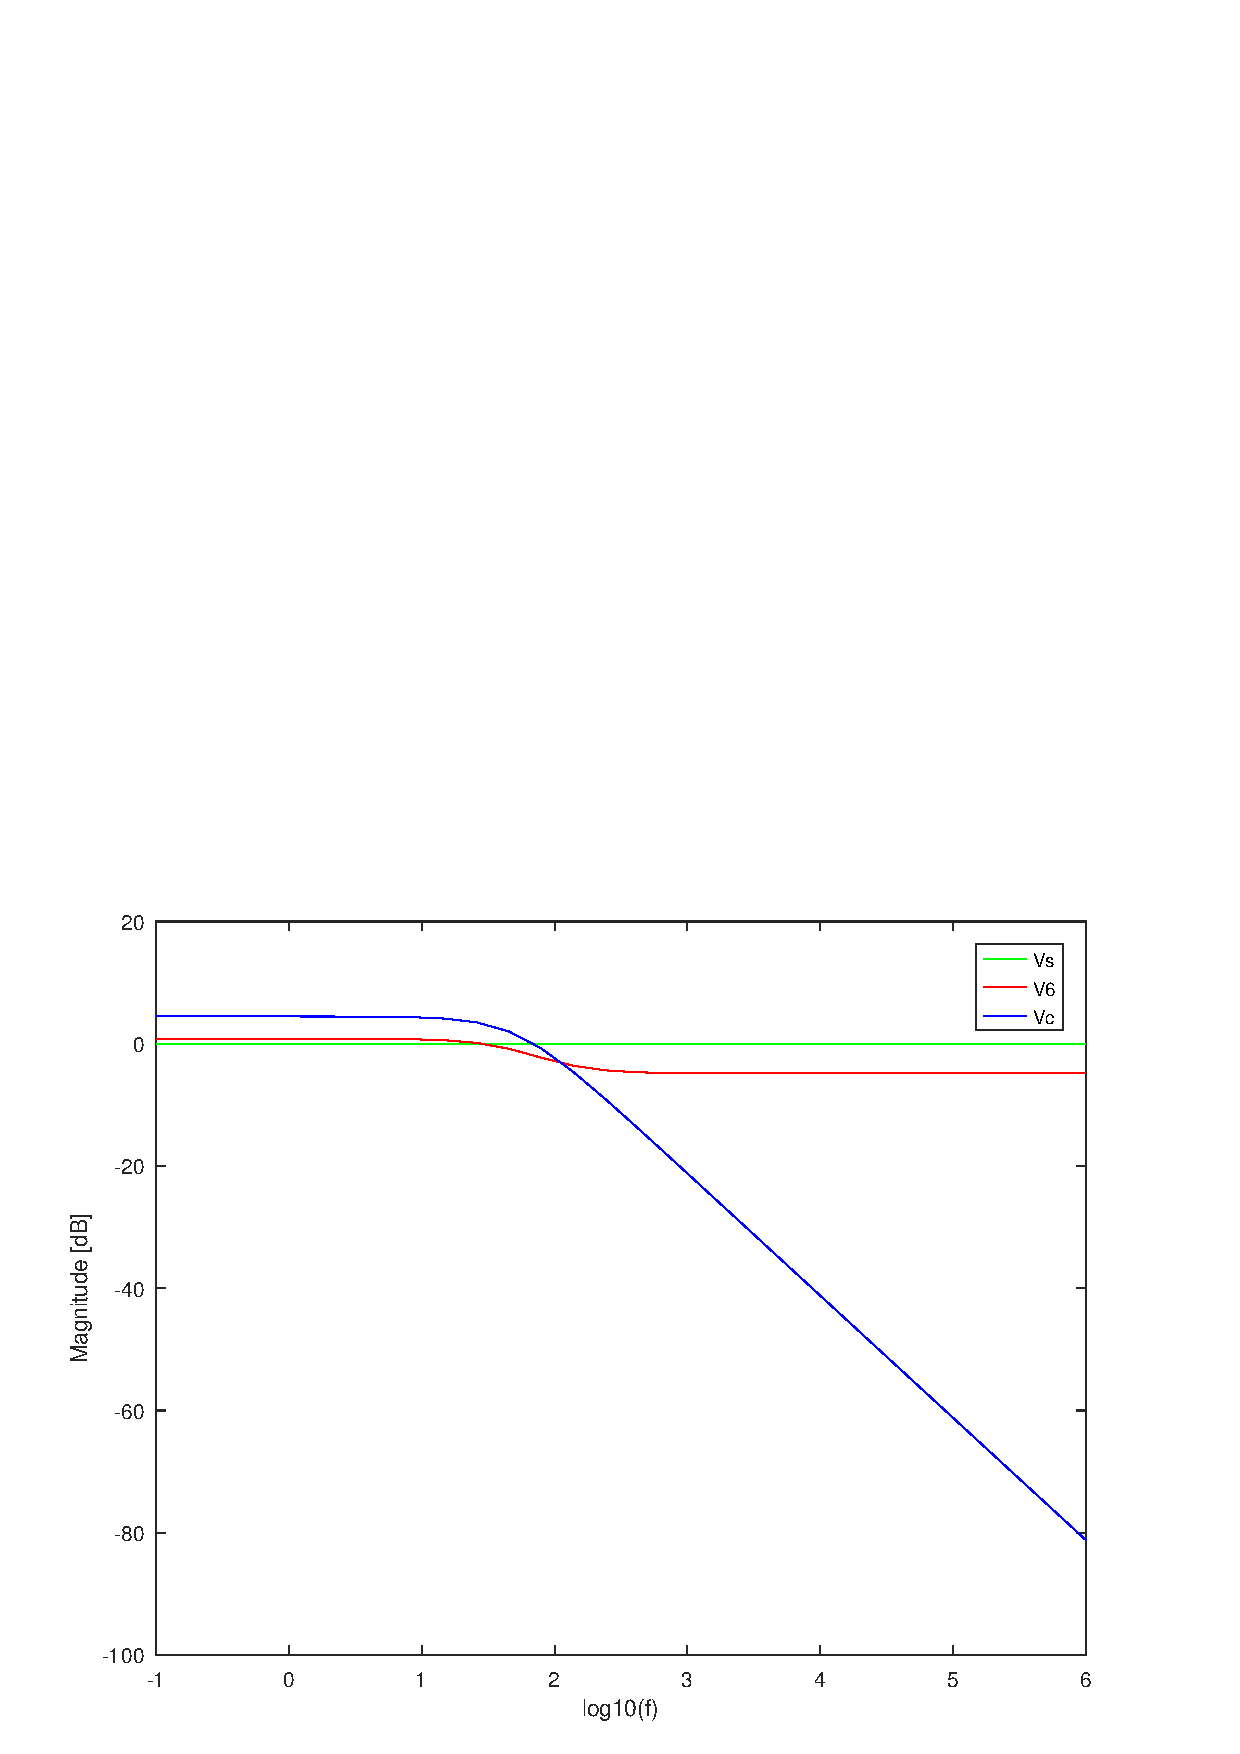
\includegraphics[width=0.6\linewidth]{magnitude.pdf}
\caption{Magnitude of $V_{s}$, $V_{c}$ and $V_{6}$ as a function of frequency}
\label{fig:magnitude}
\end{figure}
\begin{figure}[h] \centering
\includegraphics[width=0.6\linewidth]{phase.pdf}
\caption{Phase of $V_{s}$, $V_{c}$ and $V_{6}$ as a function of frequency}
\label{fig:phase}
\end{figure}
\par
